\begin{figure}
    \centering
    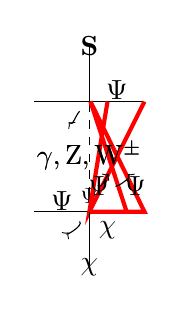
\begin{tikzpicture}[scale=.7]
        \draw[black,solid] (-1,-1) -- ++(2,0) node[midway,above,scale=.8] {$\Psi$} coordinate[pos=.5] (A); 
        \draw[black,solid] (-1,1) -- ++(2,0) coordinate[pos=.5] (B); 
        \draw[black,dashed] (A)--(B);
        \draw[red,solid,line width=1.5pt] (B)++(1,0) coordinate[pos=.99](C)--(C|-A)coordinate[pos=.67](D)--(D|-B);
        \draw[red,solid,line width=1.5pt] (A)--+(1,0) coordinate[pos=.02](E)--(E|-B)coordinate[pos=.33](F)--(F|-A);
        \draw[dashed,solid] (A)--+(0,-1);
        \draw[dashed,solid] (B)--+(0,1);        
        \draw[->] ([xshift=-.5em,yshift=-.5em]A.center) to[out=-45,in=-135] ++(-.2,-.2);
        \draw[->] ([xshift=-.5em,yshift=-.5em]B.center) to[out=-135,in=-45] ++(-.2,-.2);
        \draw[->] ([xshift=-.5em,yshift=-.5em]D.center) to[out=-45,in=-135] ++(.2,.2);
        \draw[->] ([xshift=-.5em,yshift=-.5em]F.center) to[out=-135,in=-45] ++(.2,.2);
        
        \node at ([shift={(-.5cm,.2cm)}]A.south east) {$\Psi$};
        \node at ([shift={(.5cm,.2cm)}]B.south west) {$\Psi$};
        \node at ([shift={(.5cm,-.2cm)}]D.south west) {$\Psi$};
        \node at ([shift={(-.5cm,-.2cm)}]F.south east) {$\Psi$};
        \node at ([shift={(0,1)}]B.north west) {${\bf S}$};
        \node at ([shift={(0,-1)}]B.south west) {$\gamma,\mathrm{Z},\mathrm{W}^\pm$};
        \node at ([shift={(0,1)}]A.north east) {$\gamma,\mathrm{Z},\mathrm{W}^\pm$};
        \node at ([shift={(0,-1)}]A.south east) {$\chi$};
        \node at ([shift={(0,-1)}]D.south east) {$\chi$};
    \end{tikzpicture}
    \caption{Possible UV-completion for $\mathcal{O}_3^f$ where $\chi$ (red lines) is our fermionic DM, $\Psi$ and $S$ (grey lines) are BSM particles relevant to our UV completion scenarios. The SM particles are represented by black lines.}
    \label{fig:vulcan}
\end{figure}